%%%%%%%%%%%%%%%%%%%%%%%%%%%%%%%%%%%%%%%%%%%%%%%%%%%%%%%%%%%%%%%%%%
%%%%%%%% ICML 2009 EXAMPLE LATEX SUBMISSION FILE %%%%%%%%%%%%%%%%%
%%%%%%%%%%%%%%%%%%%%%%%%%%%%%%%%%%%%%%%%%%%%%%%%%%%%%%%%%%%%%%%%%%

% Deep Network Guided Proof Search

% Use the following line _only_ if you're still using LaTeX 2.09.
%\documentstyle[icml2009,epsf,mlapa]{article}
% If you rely on Latex2e packages, like most moden people use this:
\documentclass{article}

% Employ the following version of the ``usepackage'' statement fors
% submitting the draft version of the paper for review.  This will set
% the note in the first column to ``Under review.  Do not distribute.''
\usepackage{iclr2017_arXiv,times}
\usepackage{hyperref}
\usepackage{url}

%{\"a} {\^e} {\`i} {\.I} {\o} {\'u} {\aa} {\c c} {\u g} {\l} {\~n} {\H o} {\v r} {\ss}
% & % $ # _ { } ~ ^ \
% \& \% \$ \# \_ \{ \}
% \textasciitilde
% \textasciicircum
% \textbackslash

\usepackage{tabularx}
\usepackage{multirow}

\usepackage{graphicx} % Allows including images

\usepackage{bm}
\usepackage{amsmath}
\DeclareMathOperator*{\argmin}{arg\,min}
\DeclareMathOperator*{\argmax}{arg\,max}

\usepackage{xcolor}

\usepackage{hyperref}
\hypersetup{
    colorlinks,
    citecolor=black,
    filecolor=black,
    linkcolor=black,
    urlcolor=black
}

\usepackage{multirow}

\usepackage{amssymb} % for checkmark
\usepackage{rotating} % for vertical text

\usepackage{lipsum}

%%%%%%%%%%%%%%%%%%%%%%%%%%%%%%%%%%%%%%%%%%%%%%%%%%%

%%%%%%%%%% Alex's Commands and packages %%%%%%%%%%%

%%%%%%%%%%%%%%%%%%%%%%%%%%%%%%%%%%%%%%%%%%%%%%%%%%%
\usepackage{amsthm}
\usepackage{thmtools}
\usepackage[linesnumbered,ruled,vlined]{algorithm2e} %For pseudocode

\usepackage{natbib}
%\setcitestyle{authoryear,open={[},close={]}} %Citation-related commands
%For plots
\usepackage{pgfplots}
\pgfplotsset{compat = newest}

% Define the theorem environment
\declaretheorem[style=mytheoremstyle,name=Theorem,numberwithin=section]{theorem}

% Define the corollary environment linked to the theorem
\declaretheorem[style=corlstyle,name=Corollary,numberlike=theorem,parent=theorem]{corollary}

\declaretheorem[style=corlstyle,name=Remark,numberlike=theorem]{remark}

\declaretheorem[style=corlstyle,name=Example,numberlike=theorem]{example}

% Define the lemma environment linked to the theorem
\declaretheorem[style=mytheoremstyle,name=Lemma,numberlike=theorem]{lemma}

% Define the proposition environment linked to the theorem
\declaretheorem[style=mytheoremstyle,name=Proposition,numberlike=theorem]{proposition}

% Define the definition environment linked to the theorem
\declaretheorem[style=mytheoremstyle,name=Definition,numberlike=theorem]{definition}

\usepackage{graphicx} % allow embedded images
  \setkeys{Gin}{width=\linewidth,totalheight=\textheight,keepaspectratio}
  \graphicspath{{graphics/}} % set of paths to search for images

\usepackage{listings}
\usepackage{xcolor}
\definecolor{codegreen}{rgb}{0,0.6,0}
\definecolor{codegray}{rgb}{0.5,0.5,0.5}
\definecolor{codepurple}{rgb}{0.58,0,0.82}
\definecolor{backcolour}{rgb}{0.95,0.95,0.92}
\lstdefinestyle{mystyle}{
    backgroundcolor=\color{backcolour},   
    commentstyle=\color{codegreen},
    keywordstyle=\color{magenta},
    numberstyle=\tiny\color{codegray},
    stringstyle=\color{codepurple},
    basicstyle=\ttfamily\footnotesize,
    breakatwhitespace=false,         
    breaklines=true,                 
    captionpos=b,                    
    keepspaces=true,                 
    numbers=left,                    
    numbersep=5pt,                  
    showspaces=false,                
    showstringspaces=false,
    showtabs=false,                  
    tabsize=2
}

\usepackage{wrapfig}
%%%%%%%%%%%%%%%%%%%%%%%%%%%%%%%%%%%%%%%%%%%%%%%%%%%

%%       End Alex's Commands and packages        %%

%%%%%%%%%%%%%%%%%%%%%%%%%%%%%%%%%%%%%%%%%%%%%%%%%%%

\title{An Introduction to Machine Learning}

% The \author macro works with any number of authors. There are two
% commands used to separate the names and addresses of multiple
% authors: \And and \AND.
%
% Using \And between authors leaves it to LaTeX to determine where to
% break the lines. Using \AND forces a line break at that point. So,
% if LaTeX puts 3 of 4 authors names on the first line, and the last
% on the second line, try using \AND instead of \And before the third
% author name.

\author{
  Alexandre St-Aubin \\
  %\hspace{0.5mm} attain.ai \\
  %\hspace{0.5mm} yuxili@gmail.com \\
  %\texttt{yuxili@gmail.com} \\
  }


\begin{document} 
\maketitle

\begin{abstract} 

\noindent
We discuss Machine Learning on a high level.

  \footnote{Work in progress.}

\vspace{5mm}


\textbf{Keywords:} Machine Learning


\textbf{}

\end{abstract} 


\vfill

\clearpage

\newpage

\tableofcontents

\newpage

\section{Introduction}
 
Machine learning has surged in popularity due to its ability to tackle complex problems by discerning patterns in data, making accurate predictions, and informing decisions. Unlike traditional approaches, machine learning focuses not only on understanding data but also on inferring from it, allowing models to generalize knowledge and make predictions on unseen data. This emphasis on inference enables machine learning to transcend comprehension, driving innovation and progress across various domains. There are several types of Machine Learning algorithms. The main categories are divided into \textit{Supervised learning, Semi-supervised learning, Unsupervised learning and Reinforcement learning.}

\vspace{4mm}
  \noindent \textsc{Supervised learning} allows the machine to learn through examples. The machine learning algorithm is tasked with developing the strategy for achieving the specified outputs given some input.  To do so, a known dataset is supplied  that contains a set of inputs and associated target outputs in the form $(x, t)$. The algorithm finds patterns in the data and adjusts its parameters in order to predict more accurately future inputs. This kind of machine learning algorithm needs a developer to oversee it directly. The training data must be accurately labelled. 

  The two main problems requiring Supervised learning are \textbf{Classification} and \textbf{Regression}. The former consists of classifying objects into their appropriate classes. A well known example is the MNIST data set, which is a set of images representing hand drawn numbers from 0 to 9. A classification ML algorithm will analyse each point $(x,t)$ of the data set during the \textit{training phase}, where $x$ is the image, and $t$ is the number it represents. Then, given an unseen image as input, the algorithm should predict which number it represents.

  Regression is the other common use of Supervised learning. It aims to predict a continuous output variable, rather than a discrete one (classification). An example would be to predict the cost of a house, given a set of training data consisting of characteristics of houses and their corresponding price.


\vspace{4mm}
\noindent\textsc{Semi-supervised learning} operates on a blend of labelled and unlabelled data, where labelled data contains meaningful tags for algorithmic comprehension, while unlabelled data lacks such information. By leveraging both types of data, semi-supervised learning algorithms can deduce labels for unlabelled data, enhancing their learning capability. 


\vspace{4mm}
\noindent\textsc{Unsupervised learning} algorithms discern patterns within data without predefined answers or human guidance. Through analysis, the algorithm identifies correlations and structures within datasets. Key steps in this process include clustering, which groups similar data sets, and dimension reduction, which simplifies variables to extract essential information.


\vspace{4mm}
\noindent\textsc{Reinforcement learning} involves a structured approach where algorithms are provided with actions, parameters, and goals. These algorithms explore various options, learn from trial and error, and adapt their strategies based on past experiences to optimize outcomes \citep{GuideML}.

In this paper, we will focus on \textit{Supervised learning.} However, most of the basic concepts we'll cover, such as Neurons, Neural networks, Backpropagation, and Overfitting, are topics that apply to all spheres of machine learning. 

\section{Neural Networks}
Neural networks, a subset of machine learning, form the core of supervised learning and are inspired by the human brain \citep{web:IBM:NN}. They are made of input, hidden, and output layers, and consist of interconnected \textit{neurons} with associated \textit{weights and thresholds}. Activated nodes transmit data to the next layer if their output surpasses the threshold. 
\subsection{Single Layer Perceptron} \label{sub:Single Layer Perceptron}
The simplest neural network is referred to as the perceptron. This neural network contains
a single input layer and an output node \citep{inbook:Aggarwal-1.2}.

Consider a situation where each \textit{training instance} is of the form $(\overline{X}, y)$, where each $\overline{X} = [x_1,..., x_d]$ contains $d$ feature variables, and $y \in [-1, +1]$ contains the observed value of the binary class variable. By “observed value” we refer to the fact that it is given to us as a part of the training data, and our goal is to predict the class variable for cases in which it is not observed.

%\begin{minipage}[t]{0.5\textwidth}
\begin{wrapfigure}{R}{0.4\textwidth} %this figure will be at the right
    \centering
    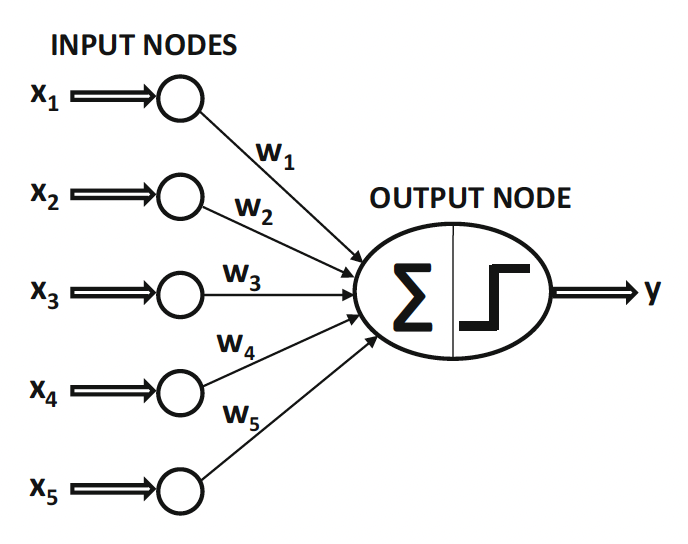
\includegraphics[width=0.4\textwidth]{SingleLayerP}
    
    \caption{A single layer perceptron.}
\end{wrapfigure}

The input layer of the \textbf{perceptron} contains $d$ nodes that transmit the $d$ features $\overline{X} = [x_1, . . . x_d]$ with \textbf{edges} of \textbf{weight} $\overline{W} = [w_1, . . . w_d]$  to an output node. The input \textbf{layer} does not perform any computation in its own right. The linear function $\overline{W} \cdot \overline{X} =\sum^{d}_{i=1}  w_ix_i$ is computed at the output node. Subsequently, the sign of this real value is used in order to predict the dependent variable of $\overline{X}$. Therefore, the prediction $\hat y$ is computed as follows:
    $$\hat y = \text{sign}[\overline{X} \cdot \overline{W}] =\text{sign}\left[\sum^{d}_{i=1}  w_ix_i\right] $$

Here, the sign function serves the role of an activation function (\ref{sub:ActivationFunction}). The goal of the \textbf{perceptron} algorithm with respect to all training instances in a data set $\mathcal{D} = \{(\overline{X_1}, y_1 ), \cdots,(\overline{X_n}, y_n )\}$ is to minimize the loss function (\ref{sub:Loss Function}). We shall learn more about loss functions in a following section, but an example would be to minimize the least-squares function: 
 \begin{equation*}
  \begin{split}
    \sum^{n}_{i=1} (\hat y_i - y_i)^2 =\sum^{n}_{i=1} \left(\text{sign}[\overline{X_i} \cdot \overline{W}] -y_i \right)
  \end{split}
 \end{equation*}

 To optimize the loss function, the perceptron will use a \textit{gradient descent} method, which we will see later.
 \subsection{Neurons}%
  \label{sub:Neurons}
The neuron is the smallest computational unit of a neural network. The single layer perceptron described in the previous section is exactly a neuron.  
\begin{definition}[Neurons]
  Neurons are made up of 4 elements: 
  \begin{enumerate}
    \item The inputs, seen as \textit{nodes}, consist of either the input layer (\autoref{sub:Layers}), or the outputs of the previous layer of the neural network. 
    \item The weights (\autoref{def:weight}) and biases (\autoref{def:bias}), seen as \textit{edges} will act on the outputs of previous neurons before they reach the input function of the neuron. 
    \item The input function takes a sum of the weighed inputs. 
    \item The activation function (\autoref{sub:ActivationFunction}) acts on the input function and outputs the result to the following layers. 
  \end{enumerate}
   A simple mathematical model for a neuron's output activation is \citep{book:AIModernApp}
  \begin{figure}
    \centering
    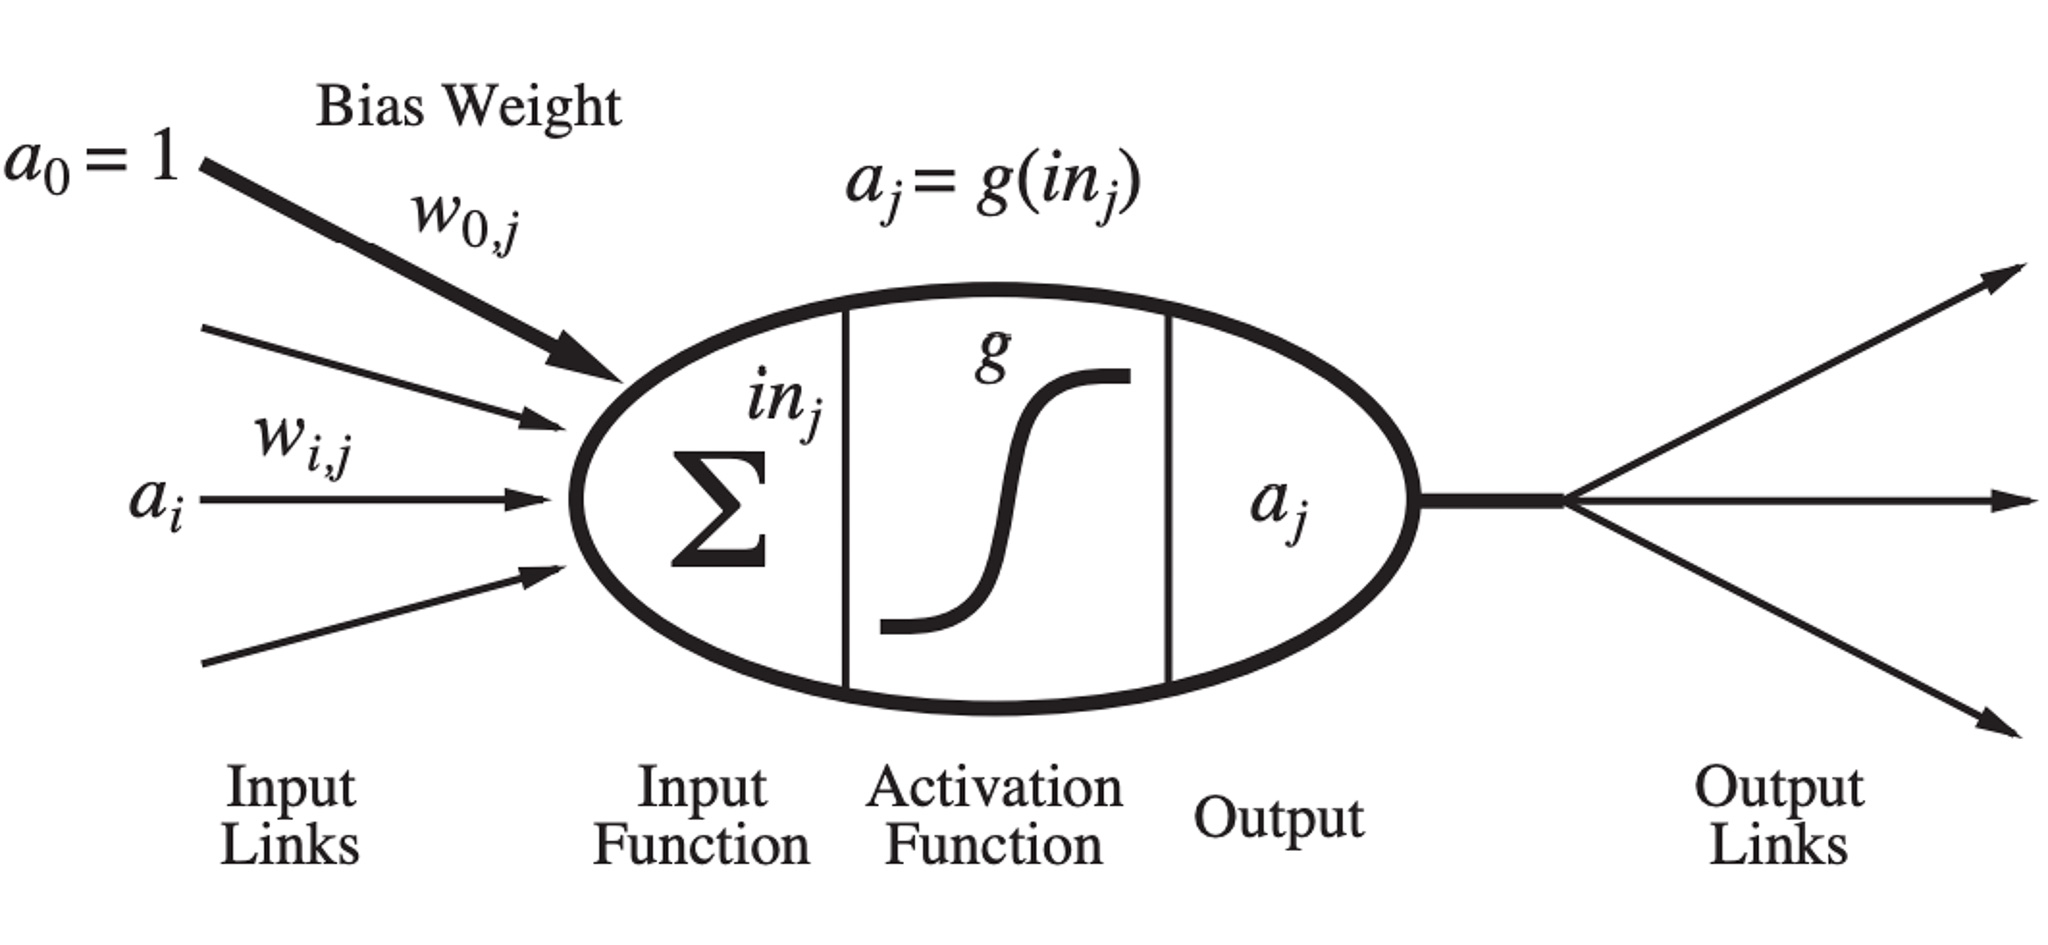
\includegraphics[width=0.75\textwidth]{Neuron}
  \label{Neuron}
  \caption{A neuron and its inputs and outputs.}
\end{figure}
  $$o_j = f \left( \sum^{n}_{i=0}w_{i,j} o_i  \right)$$
  where $f$ is the activation function, $o_i$ is the output activation of neuron $i$ and $w_{i,j}$ is the weight on the directed edge from neuron $i$ to the neuron $j$. 
\end{definition}
\begin{definition}[Weights]\label{def:weight}
  A weight $w_{i,j} \in \mathbb{R}$ will multiply the output of neuron $i$ before giving it as input to neuron $j$. Weights are the moving parts of the neural network, as they get changed during each iteration of the learning step in order to optimize the output. They can be initialized to any random value, and after running the network on a pair $(x,t)$ from the \textit{training data}, the weight update rule (\autoref{sub:Weight Update Rule}) will alter them to minimize the error between the output $\hat y$ and the target $t.$ 
\end{definition}
\begin{definition}[Bias]\label{def:bias}
  Biases are constant, they are an additional input into the next layer that will always have the value of 1. Bias units are not influenced by the previous layer but they do have outgoing connections with their own weights. The bias unit guarantees that even when all the inputs are zeros there will still be an activation in the neuron \citep{WeightsBias}. 
\end{definition}
\subsection{Feed-Forward Neural Networks}%
  \label{sub:Feed-Forward Neural Networks}
  Having defined neurons, the building blocks of neural networks, we may now give a rigorous definition of the latter. A feed-forward network has connections only in one direction—that is, it forms a directed acyclic graph. Every node receives input from “upstream” nodes and delivers output to “downstream” nodes; there are no loops. A feed-forward network represents a function of its current input; thus, it has no internal state other than the weights themselves \citep{book:AIModernApp}.

The overall network is a combination of function composition and matrix multiplication:

  $$g(x) = f^L (W^Lf^{L-1}(W^{L-1} \hdots f^1(W^1x)\hdots)), $$
  where $L$ is the number of layers (\autoref{sub:Layers}), $W$ is the weight matrix, and $f$ is the activation function (\ref{sub:ActivationFunction}).
 \begin{definition}[Feed-forward Neural Network]
  A neural network is a \textit{computational directed acyclic graph,} in which a unit of computation is the neuron. Each directed edge in the graph represents a function passing the weighed output of a node in a layer to a node in the next layer.
 \end{definition} 

   Artificial neural networks are often refered to as \textbf{multi-layer perceptrons} (abbreviated to MLPs) for one simple reason: you can think of such an MLP as the composition of multiple perceptrons, where, in this case, the perceptron would be a synonym for artificial neuron, so the smallest computational unit of a neural network, which performs, for example, a linear combination of its inputs followed by the application of an activation function, which can be the sigmoid, tanh, ReLU, identity, or any other function that is differentiable, if you plan to train the neural network with gradient descent.
\subsection{Layers}
\label{sub:Layers}
Feed-forward networks are usually arranged in layers, such that each unit receives input
only from units in the immediately preceding layer. The layers are divided in 3 groups: the \textit{input, hidden,} and \textit{output} layers. Layers are a general term given to a grouping of neurons that act together in the neural network.
  \begin{wrapfigure}{R}{0.4\textwidth} %this figure will be at the right
    \centering
    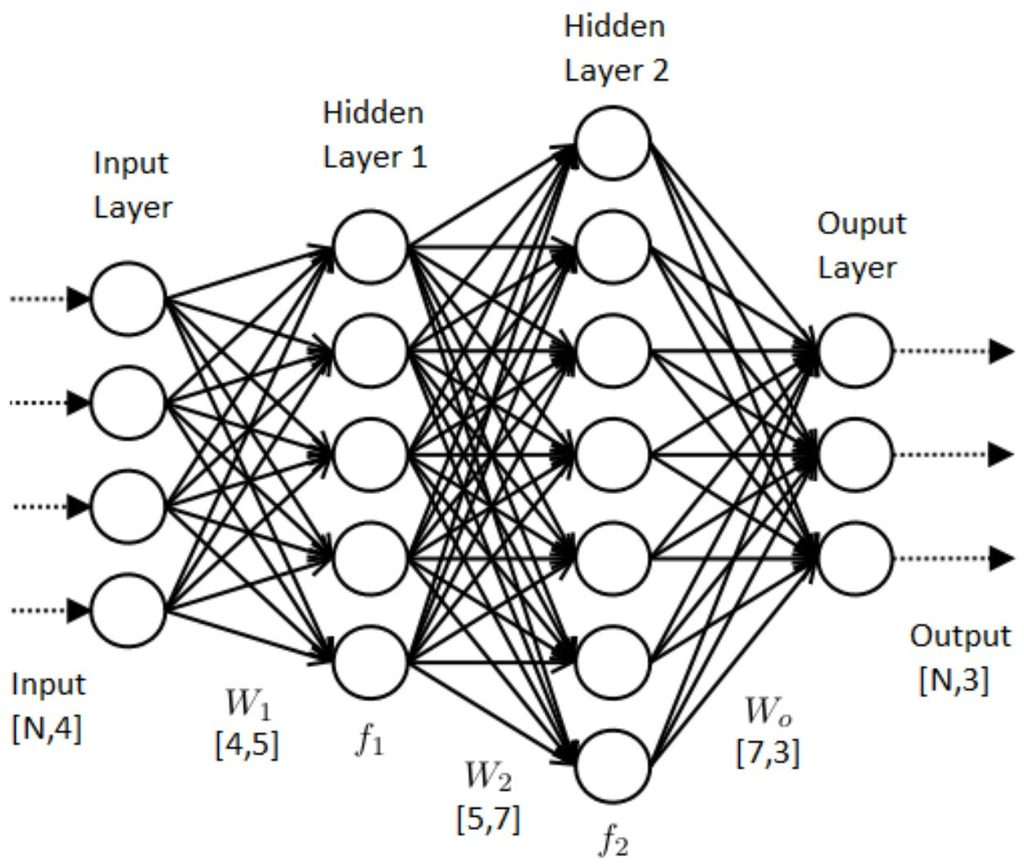
\includegraphics[width=0.4\textwidth]{NeuralNetwork}
    \caption{A graph representation of a Neural Network.}
\end{wrapfigure}

The first layer in a neural network is the \textbf{Input Layer}, it receives the initial data for the network from the outside world. The "Entry point" of the neural network. Then, come the \textbf{hidden layer(s)}, which are where the magic happens in neural networks. Each layer is trying to learn different aspects about the data by minimizing the \textbf{cost function}. The most intuitive way to understand these layers is in the context of image recognition such as a face. The first layer may learn edge detection, the second may detect eyes, third a nose, etc. \citep{layers}. The final layer in the neural network is the \textbf{output layer}. This layer is responsible for holding the final result or output of the problem. Input, such as raw images, is fed into the input layer, and the output layer produces the corresponding result.


\subsection{Activation Function}%
  \label{sub:ActivationFunction}
An activation function in neural networks is a smooth function applied to the output of each neuron in a layer. It introduces non-linearity to the network, allowing it to learn complex patterns and relationships in the data.

The activation function determines whether a neuron should be activated or not based on the weighted sum of its inputs. In other words, it defines the output of a neuron given a set of inputs. Without activation functions, neural networks would be limited to linear transformations, and they wouldn't be able to capture the non-linearities present in many real-world datasets. 

\vspace{5mm}
\noindent \textbf{Desired Characteristics of Activation Functions} \citep{jagtap2022important}

\noindent There is no universal rule for choosing the best activation function, but there are some characteristics to look for, namely
\begin{enumerate}
  \item \textbf{Nonlinearity} is one of the most essential characteristics
of an activation function is nonlinearity. In comparison
to linear activation functions, the non-linearity of the
activation function significantly improves the learning
capability of neural networks. 
\item The activation function must
  be \textbf{computationally cheap}. This has
the potential to greatly improve network efficiency.
  \item It must be \textbf{bounded}, as gradient-based training approaches are more stable when the range of the activation function is finite, because pattern presentations
significantly affect only limited weights. 
\item The most desirable quality for using
gradient-based optimization approaches is \textbf{continuously
  differentiable} activation functions. This ensures that the
back-propagation algorithm works properly. 
\end{enumerate}
\begin{remark}[The vanishing and exploding gradient problems] The variation
of the inputs and outputs of some activation functions,
such as the logistic function (Sigmoid), is extremely
large. To put it another way, they reduce and transform
a bigger input space into a smaller output space that
falls between [0,1]. As a result, the back-propagation
algorithm has almost no gradients to propagate backward
in the network, and any residual gradients that do exist
continue to dilute as the program goes down through the
top layers. Due to this, the initial hidden-layers are left
with no information about the gradients. For hyperbolic
tangent and sigmoid activation functions, it has been
observed that the saturation region for large input (both
positive and negative) is a major reason behind the
vanishing of gradient. One of the important remedies
to this problem is the use of non-saturating activation
functions, such as ReLU.
\end{remark}
We present some commonly used activation functions.
\begin{enumerate}
  \item \textit{Sigmoid Function.} Its range is $[0,1]$, and is defined as,
$$\sigma(x) = \frac{1}{1 + e^{-x}}$$
Advantage: boundedness. \\ Disadvantages:
the vanishing gradient problem, the output not being zerocentered, and the saturation for large input values. 
  \item \textit{Hyperbolic Tangent Function.} It is mostly used for
regression problems, has a range of $[-1,1]$, and is defined as,
$$\tanh(x) = \frac{e^{x} - e^{-x}}{e^{x} + e^{-x}}$$
Advantage: zerocentered structure. \\
Disadvantage: the vanishing gradient problem, i.e. once saturated, it is really challenging
for the learning algorithm to adapt the parameters and learn
faster.
  \item \textit{ReLU Function.} ReLU was primarily used to overcome the vanishing gradient problem. ReLU is the most common activation function used for \textit{classification problems}. Its range is $[0, \infty)$, and is defined as
  $$\text{ReLU}(x) = \max(0, x)$$
Advantages: Apart from overcoming the vanishing gradient problem, the
implementation of ReLU is very easy and thus cheaper, unlike
tanh and sigmoid, where an exponential function is needed.
\\
Disadvantages: It has a saturation region, which can prevent the
learning of the networks. In particular, ReLU always discards
the negative values, which makes the neurons stop responding to
the gradient-based optimizer. This problem is known as \textit{dead
or dying ReLU problem}, meaning the neurons stop
outputting other than zero. 
  \item \textit{Softplus Function.} It approximates the ReLU activation function in a smooth way, with a range of $(0, \infty)$, and it is defined as
$$\text{Softplus}(x) = \ln (1+ e^x) $$
  \item \textit{Softmax.} It is a generalization of logistic
function in high dimensions. It normalizes the output and
divides it by its sum, which forms a probability distribution. The standard softmax function Softmax$: \mathbb{R}^k \to (0,1)^k$ is defined as 
$$\text{Softmax}(x_i) = \frac{e^{x_i}}{\sum^{k}_{j=1} e^{x_j}} \quad \text{for } i= 1,...,k   $$
In other words, it applies
the standard exponential function to each element $x_i$
of the input vector $x$ and normalizes these values by
dividing them by the sum of all these exponentials, which ensures that the sum of the components of the output vector is 1.
\end{enumerate}
\begin{figure}[b]
  \label{actfun}
  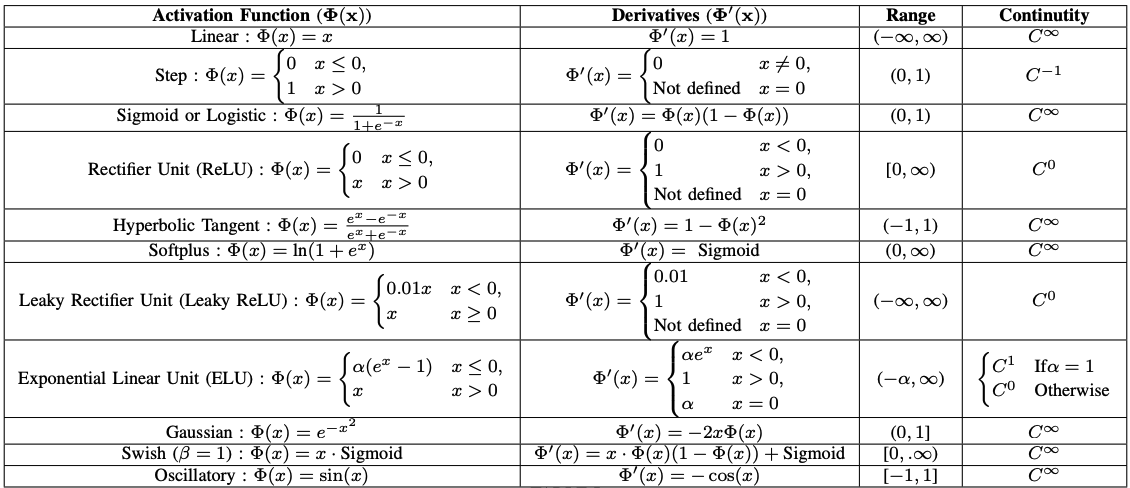
\includegraphics{ActFunTable}
\caption{Common activation functions, their derivatives, range, and order of continuity.}
\end{figure}

\newpage
\section{Learning}
  \label{sec:Learning}
  At the core of machine learning lies the art of learning itself. In this section, we delve into the essential components that drive this process forward: backpropagation, loss functions, and the delicate balance of model fitting.

Backpropagation serves as the engine of learning in neural networks, refining model parameters through the propagation of error starting from the output, all the way to the first hidden layer. Accompanying this is the concept of loss functions, which quantify the disparity between predicted and actual outcomes, guiding the learning trajectory towards convergence.

In the subsections ahead, we dissect each facet of learning, providing insights into backpropagation, weight update rules, and unraveling the nuances of loss functions.\subsection{BackPropagation}%
  \label{sub:BackPropagation}
\textbf{Backpropagation} is a gradient estimation method used to train neural network models. The gradient estimate is used by the optimization algorithm to compute the network weight updates. So, when we say a neural network is \textit{learning}, it means that backprop is computing a gradient descent that minimizes the loss function, and updates the weights using a \textbf{weight update rule} \ref{sub:Weight Update Rule}. Backpropagation is a way of computing the partial derivatives of a loss function with respect to the weights of a network; we use these derivatives in gradient descent, exactly the way we would with linear regression and logistic regression. 
\begin{wrapfigure}{r}{0.4\textwidth} %this figure will be at the right
    \centering
    \label{simpleNet}
    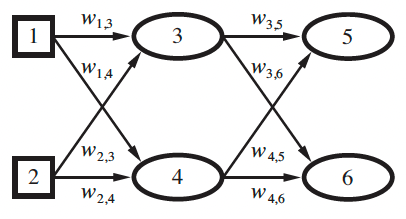
\includegraphics[width=0.4\textwidth]{simpleNet}
    \caption{A simple network with 2 inputs, one hidden layer, and two outputs.}
\end{wrapfigure}
  Let us first begin by recalling that a neural network evaluates compositions of functions computed at individual nodes. Think of a neural network as a function $h_w(x)$ of the input, parametrized by the weights. Consider the network in Figure 5, let $\{x_1,x_2\}$ be the input vector, $f$ the activation function and $a_i$ denote the activated output at node $i$. Then, the output at node 3 is given by
  $$a_3 = f(w_{0, 3} + f(x_1)w_{1,3} + f(x_2)w_{2,3}), $$
  where $w_{0,3}$ is the bias weight (\autoref{def:bias}) at node 3. Similarly, the output at node 5 is
  \begin{equation*}
    \begin{split}
      a_5 &= f( w_{0,5} + f(a_3) w_{3,5} + f(a_4) w_{4,5}  )\\ 
      &= f[w_{0,5} + f(w_{0, 3} + f(x_1)w_{1,3} + f(x_2)w_{2,3})w_{3,5} +f(w_{0, 4} + f(x_1)w_{1,4} + f(x_2)w_{2,4})w_{4,5} ]
    \end{split}
  \end{equation*}
  And even with such a small network, we can already see how awkward it would be to compute the derivative of $a_5$ with respect to $w$. But an even bigger problem arises when we think of how we would compute the loss function in hidden layers. Whereas the error $y -h_w$\sidenote{$y$ is the target output, and $h_w$ the value computed by the network } at the output layer is clear, the error at the hidden layers seems mysterious because the training data do not say what value the hidden nodes should have.
\begin{wrapfigure}{r}{0.4\textwidth} %this figure will be at the right
    \centering
    \label{simpleNet}
    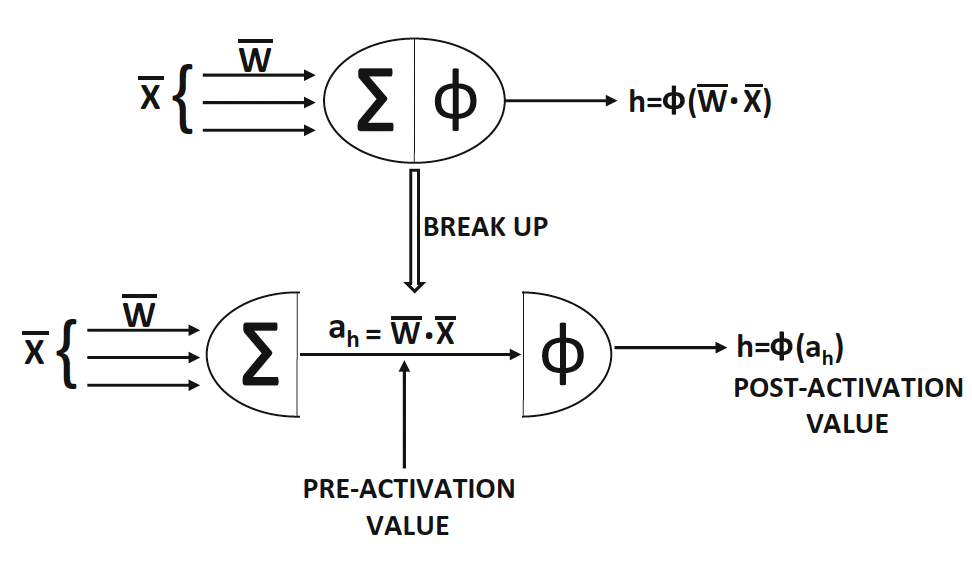
\includegraphics[width=0.4\textwidth]{pre-post-neuron}
    \caption{Pre and Post activation values of a neuron.}
\end{wrapfigure}

  Therefore, we need some kind of iterative approach to compute the derivatives, and a way to \textit{back-propagate} the error from the output layer to the hidden layers. The resulting iterative approach uses \textit{dynamic programming}, and the \textbf{weight update rule} is the \textit{chain rule} of differential calculus \citep{inbook:Aggarwal-3.2}.

\begin{theorem}[Multivariate Chain Rule] \label{chain}
    Let $z = f(y_1, y_2, \ldots, y_m)$ be a differentiable function of $m$ variables, where each $y_j = g_j(x_1, x_2, \ldots, x_n)$ is a differentiable function of $n$ variables. Then, for each $i = 1, 2, \ldots, n$, the partial derivative of $z$ with respect to $x_i$ is given by
$$
\frac{\partial z}{\partial x_i} = \sum_{j=1}^{m} \frac{\partial z}{\partial y_j} \frac{\partial y_j}{\partial x_i}.$$
  \end{theorem}
  We note that backpropagation can be implemented by using either the \textit{pre-activation}, or \textit{post-activation} values at each neuron. Here, we'll focus on the method that acts on the pre activation values neurons. For the sake of simplicity, we view the neural network as a \textit{Directed Acyclic Graph} $G$, where 
  \begin{enumerate}
    \item Each node represents a neuron, and is denoted by a number $j$.
    \item The weight on the edge from neuron $i$ to $j$ is denoted $w_{i,j}$.
  \end{enumerate}
  The algorithm can be divided in two phases: \textit{forward} and \textit{backward}.
  \begin{enumerate}
    \item \textbf{Forward Phase.} The term "forward phase" refers to this process of computing values of each hidden layer depending on the current weight values using a specific input vector. These computations naturally cascade forward across the layers. The aim of the forward phase is to compute every intermediate hidden and output variable for a given input. The Backward phase will call for these values. The derivative of the loss function $L$ with respect to this output, as well as the value of the output $o$, are calculated at the completion of the computation. For the sake of simplicity, we will explore the case of a single output node for the time being. We will then talk about the simple generalization to many outputs. 

    \item \textbf{Backward Phase.} In this phase, the gradient of the loss function with respect to different weights is calculated. First, the derivative $\frac{\partial {o}}{\partial {w}} {}$ is computed. This establishes the gradient computation's initialization. The multivariable chain rule is then used to propagate the derivatives in the opposite direction. Since we are focussing on the pre-activation approach, the gradients are computed with respect to the pre-activation values of the hidden variables, which are then propagated backwards.
  \end{enumerate}
  More precisely, the process can be described as follows. Let $(x,t)$ be the input to our algorithm, where $t$ is the target output of the input vector $x.$ Define the value
  $$L = \operatorname{Loss}(y,t),$$
  where Loss could be any \textit{loss function}, such as the MSE. At each neuron $j$, let its post-activation output be 
  $$o_j = \Phi (\net_j) = \Phi \left( \sum^{n}_{i=0}w_{i,j} o_i  \right) , $$
  where $\Phi$ is any \textit{activation function}, $w_{i,j}$ is the weight on the edge between neurons $i$ and $j$, and $o_i$ is the output from neuron $i.$ Then, the pre-activation value is easily seen to be $\net_j$.

  \begin{enumerate}
    \item The \textbf{forward pass} propagates $x$ through the neural network, computing the values of all hidden neurons to reach the output $\hat y$ of the neural network, which corresponds to the predicted output. Then, $L = \operatorname{Loss}(\hat y, t)$  is computed.
    \item The derivative $\frac{\partial {L}}{\partial {\hat y}}$ at the output can be directly computed. Then, to compute the derivative of $L$ with respect to $o_j$ for an arbitrary neuron $j$, 

    \item Consider $L$ as a function of all neurons receiving input from $j$, and denote this set by $I_j =\{ i_1^{(j)}, ..., i_n^{(j)}\}$. Then, 
    $$\frac{\partial {L(o_j)}}{\partial {o_j}} = \frac{\partial {L(\net_{i_1^{(j)}}, ..., \net_{i_n^{(j)}})}}{\partial {o_j}} {} $$
    to obtain the following recurrence relation for the derivative of $L$ with respect to $o_j$, by the chain rule, 
    \begin{equation}\label{deriv_o_j}
      \begin{split}
        \frac{\partial {L}}{\partial {o_j}} = \mathlarger{\mathlarger{\sum}}^{}_{i \in I_j} \left( \frac{\partial {L}}{\partial {\net_i}} \frac{\partial {\net_i}}{\partial {o_j}}  \right)  =&  \mathlarger{\mathlarger{\sum}}^{}_{i \in I_j} \left( \frac{\partial {L}}{\partial {o_i}} \frac{\partial {o_i}}{\partial {\net_i}} \frac{\partial {\net_i }}{\partial {o_j}} \right) \\ =&\mathlarger{\mathlarger{\sum}}^{}_{i \in I_j} \left( \frac{\partial {L}}{\partial {o_i}} \frac{\partial {o_i}}{\partial {\net_i}} w_{j,i}\right) 
      \end{split}
    \end{equation}
    We can see that the derivative with respect to $o_j$ can be computed if those of the neurons on the next layer are already known, per the \textit{recurrent} behaviour of this algorithm. 
    \item We now have all the necessary tools to compute the partial derivative of $L$ with respect to the weight $w_{i,j}$. Again, by applying the chain rule, we get
    \begin{equation}\label{deriv_w}
  \begin{split}
    {\frac {\partial L}{\partial w_{i,j}}}={\frac {\partial L}{\partial o_{j}}}{\frac {\partial o_{j}}{\partial w_{i,j}}}=&{\frac {\partial L}{\partial o_{j}}}{\frac {\partial o_{j}}{\partial {\text{net}}_{j}}}{\frac {\partial {\text{net}}_{j}}{\partial w_{i,j}}}\\ 
    =& {\frac {\partial L}{\partial o_{j}}}{\frac {\partial o_{j}}{\partial {\text{net}}_{j}}} \left(\frac{\partial {}}{\partial {w_{ij}}} {\sum^{n}_{k=1} w_{k,j}o_k}\right) \\ 
    =&{\frac {\partial L}{\partial o_{j}}}{\frac {\partial o_{j}}{\partial {\text{net}}_{j}}} \left(\frac{\partial {w_{i,j} o_i}}{\partial {w_{i,j}}} \right)={\frac {\partial L}{\partial o_{j}}}{\frac {\partial o_{j}}{\partial {\text{net}}_{j}}} o_i
  \end{split}
\end{equation}
   and so, we may consider the following recursively defined function to simplify notation,

\begin{equation*}
  \begin{split}
    \delta_j = {\frac {\partial L}{\partial o_{j}}}{\frac {\partial o_{j}}{\partial {\text{net}}_{j}}}= 
    \begin{cases}
      \frac{\partial {L(t, o_j)}}{\partial {o_j}} \frac{d {\varphi (\net_j)}}{d {\net_j}}, &\text{ if } j \text{ is an output neuron, }\\
      \left( \sum^{}_{i\in I_j} w_{j,i} \delta_i\right) \frac{d {\varphi (\net_j)}}{d {\net_j}} {}, &\text{ otherwise.} 
    \end{cases}
  \end{split}
\end{equation*}
to conclude that the partial derivative of $L$ with respect to the weight $w_{i,j}$ is given by 
\begin{equation*}
  \begin{split}
    \frac{\partial {L}}{\partial {w_{i,j}}} = o_i \delta_j
  \end{split}
\end{equation*}
      \end{enumerate}
\subsection{Weight Update Rule}%
  \label{sub:Weight Update Rule}
  After having found the derivatives of the loss function with respect to the weights, one needs a way to update the weights. The goal is to modify the weights of the neural network so that given the input $(x,t)$, where $x$ is the input vector and $t$ the target output, it points more toward $t$. Then, in the future, it will have a better chance of classifying $x$ correctly \citep{Hagan_Martin}. The naive way would be to set the weights so that they point directly to $t$. Unfortunately, this leads to overfitting, which we'll address in the next chapter.
  
  To update the weight $w_{i,j}$ using backpropagation, we first choose a learning rate $\mu> 0$. We may then choose to update $w_{i,j}$ by adding $\Delta w_{i,j}$ to it, where
  \begin{equation*}
    \begin{split}
      \Delta w_{i,j} = -\mu \frac{\partial {L}}{\partial {w_{i,j}}}  = - \mu  o_i \delta_j
    \end{split}
  \end{equation*}
 Then, the weight update rule would be defined as, 
 \begin{equation*}
  \begin{split}
    w_{i,j}^{(\text{updated})} =  w_{i,j}^{(\text{old})} - \mu  o_i \delta_j
  \end{split}
 \end{equation*}
 We claim that this update rule decreases the loss $L$. 
 \begin{proof} 
  
If ${\frac {\partial L}{\partial w_{i,j}}}>0$, an increase in $w_{i,j}$ increases $L$; conversely, if $\frac {\partial L}{\partial w_{i,j}}<0$, an increase in $w_{i,j}$ decreases $L$. The new $\Delta w_{i,j}$ is added to the old weight, and the product of the learning rate and the gradient, multiplied by $-1$ guarantees that $w_{i,j}$  changes in a way that always decreases $L$. 
 \end{proof}

\subsection{Regression Loss Functions}%
  \label{sub:Loss Function}
  The attentive reader will have noticed that supervised machine learning revolves around optimizing the outputs of a loss function. This also applies to a wide range of other machine learning strategies. Thus, defining a good loss function is essential. We offer an overview of the most widely utilized loss functions for a variety of uses, starting with \textbf{Regression Losses}.


  Regression losses are loss functions used to solve the regression problems of \textit{supervised ML}. Recall that regressions model predict the output of a continuous output variable. The regression losses are all based on residuals, namely the difference between the predicted and expected outputs. In the following, let $x_i$ be the $i^{th}$ element of input $x$, $f(x_i)$ the $i^{th}$ element of the predicted output, and $y_i$ the $i^{th}$ element of the expected output. The following represent commonly used regression losses,
  \begin{enumerate}
    \item \textit{Mean Bias Error Loss [Continuous, Differentiable]}. The Mean Bias Error loss is the most basic loss function, it is given by,
    \begin{equation}
      \begin{split}
        \mathcal{L}_{MBE} (y_i, f(x_i))= \frac{1}{n} \sum^{n}_{i=1} [y_i-f(x_i)]
      \end{split}
    \end{equation}
 It measures the average bias in the prediction, but because positive errors have the ability to cancel out negative ones and create an incorrect parameter estimate, it is rarely used as the loss function to train regression models. However, it serves as the foundation for the ensuing loss functions and is frequently employed to assess the models' performances \citep{ciampiconi2023survey}.
    \item \textit{Mean Absolute Error Loss (L1) [Lipschitz-Continuous, Convex].} The Mean Absolute Error loss is one of the most fundamental loss functions for regression; it measures the average of the absolute bias in the prediction. The absolute value overcomes the problem of the MBE by ensuring that positive errors do not cancel the negative ones. It is defined as, 
    \begin{equation}
      \begin{split}
        \mathcal{L}_{MAE}(y_i, f(x_i)) = \frac{1}{n} \sum^{n}_{i=1} |y_i-f(x_i)|
      \end{split}
    \end{equation}

    Notice that the contribution of the errors follows a linear behaviour, implying that many small errors have as much impact as a big one. This implies that the gradient magnitude is not dependent on the error size, thus leading to convergence problems when the error is small. A model trained to minimize the MAE performs well when the target data conditioned on the input is symmetric \citep{ciampiconi2023survey}.
    \item \textit{Mean Squared Error Loss (L2) [Continuous, Differentiable, Convex].} The Mean Squared Error loss is a well-known and simple loss function for regression. It is given by 
    \begin{equation}
      \begin{split}
        \mathcal{L}_{MSE}(y_i, f(x_i)) = \frac{1}{n} \sum^{n}_{i=1} (y_i-f(x_i))^2
      \end{split}
    \end{equation}
The squared term makes all the biases positive and magnifies the contribution made by outliers, making it more suitable for problems where noise in the observations follows a normal distribution. The sensitivity to the outliers is the primary disadvantage \citep{ciampiconi2023survey}.
    \item \textit{Root Mean Squared Error Loss [Continuous, Differentiable, Convex].} The Root Mean Squared Error loss is, apart from the square root term, identical to MSE. It main benefit is that the loss has the same units and scale as the relevant variable. The minimization procedure converges to the same optimal value as MSE. However, the RMSE may take different gradient steps depending on the optimization method employed \citep{ciampiconi2023survey}. It is defined as, 
    \begin{equation}
      \begin{split}
        \mathcal{L}_{RMSE}(y_i, f(x_i)) = \sqrt{\frac{1}{n} \sum^{n}_{i=1} (y_i-f(x_i))^2}
      \end{split}
    \end{equation}
    \item \textit{Huber Loss [Lipschitz-Continuous, Differentiable, Strictly Convex].} Huber loss is a mix of MAE and MSE. When the residuals are sufficiently small, it goes from MAE to MSE. It is parameterized by $\delta$, which indicates the point at which MAE and MSE transition. This enables it to combine the benefits of the MAE and the MSE. When there is a significant discrepancy between the model's output and prediction, the Huber loss becomes less susceptible to outliers since the errors are linear. On the other hand, if the error is tiny, it follows the MSE, which accelerates convergence and makes it differentiable at $0$. A crucial decision is which $\delta$ to use, which may be modified often throughout the training process depending on what constitutes an outlier \citep{ciampiconi2023survey}. The Huber loss is given by,
\begin{equation}
      \begin{split}
        \mathcal{L}_{Huber}(y_i, f(x_i)) = \sum^{n}_{i=1} \alpha_i(y_i, f(x_i)),
      \end{split}
    \end{equation}
    where, 
    \begin{equation*}
      \begin{split}
        \alpha_i(y_i, f(x_i)) =\begin{cases}
          \frac{1}{2} (y_i-f(x_i))^2, &\text{ if } |y_i -f(x_i) | \leq \delta \\  
          \delta\left( |y_i -f(x_i)| -\frac{1}{2}\delta \right), &\text{ otherwise.} 
        \end{cases}
      \end{split}
    \end{equation*}
    \item \textit{Log-cosh Loss [Continuous, Differentiable].} The Log-cosh loss is given by the logarithm of the \textit{hyperbolic cosine} of the residuals between the actual value $y$ and the forecasted value $f(y_i)$. It is more computationally demanding than \textit{Huber loss}, but it provides all the same benefits without the need to establish a hyperparameter. Moreover, the log-cosh loss has the advantage of being twice differentiable, which makes it appropriate for techniques that need to solve the second derivative \citep{ciampiconi2023survey}. It is defined as, 
  \begin{equation}
      \begin{split}
        \mathcal{L}_{Logcosh}(y_i, f(x_i)) = \frac{1}{n} \sum^{n}_{i=1} \log[\cosh(y_i-f(x_i))]
      \end{split}
    \end{equation}
    \item \textit{Root Mean Squared Logarithmic Error Loss [Continuous, Differentiable, Convex].} The Root Mean Squared Logarithmic Error (RMSLE) loss is given by,
\begin{equation}
      \begin{split}
        \mathcal{L}_{RMSLE}(y_i, f(x_i)) = \sqrt{\frac{1}{n} \sum^{n}_{i=1} [\log (y_i + 1) - \log(f(x_i)+1)]^2 }
      \end{split}
    \end{equation}

     When it comes to RMSE, the only distinction is that the logarithm is used on both the observed and the anticipated values. The logarithm's plus one term permits zero values for $f(x_i)$. The RMSLE is more resilient to outliers because of the logarithm, as well as the relative inaccuracy between the expected and actual values. In particular, the RMLSE's size does not increase in proportion to the error's magnitude. Rather, when both the anticipated and actual values are high, data points with large residuals are not penalized as much. Because of this, the RMSLE is a viable option for problems where the targets have an exponential relationship or when penalizing underestimates more heavily than overestimates is desirable. This loss, however, is inappropriate for problems where negative values are permitted \citep{ciampiconi2023survey}.
  \end{enumerate}
\subsection{Classification Loss Functions}%
  \label{sub:Classification Loss Functions}
  The second subset of supervised ML, \textit{Classification}, also has its own set of loss functions. The following consists of the most commonly used \textit{Margin-based} Classification losses. 
  \begin{enumerate}
    \item \textit{Zero-one Loss.} The Zero-one loss is the most basic classification loss function. It is defined as, 
    \begin{equation}
      \begin{split}
        \mathcal{L}_{Zero-One}(y, f(x)) = 
        \begin{cases}
          1, &\text{ if } f(x) \cdot y < 0 \\ 
          0, &\text{ otherwise.} 
        \end{cases}
      \end{split}
    \end{equation}
    In practice, the Zero-one loss can't be used since it is not convex, nor differentiable.
    \item \textit{Hinge Loss [Lipschitz-continuous, Convex].} The Hinge loss is among the most famous loss functions for classification. It is given by, 
 \begin{equation}
      \begin{split}
        \mathcal{L}_{Hinge}(y, f(x)) = \max(0, 1-f(x)\cdot y)
      \end{split}
    \end{equation}
    The two main drawbacks of Hinge loss are that it is sensible to outliers, and that its derivative is discontinuous at $f(x)\cdot y = 1$. The latter makes it harder to optimise.
    \item \textit{Quadratically Smoothed Hinge Loss [Lipschitz-continuous, Convex, Differentiable].} The Quadratically Smoothed Hinge loss is a smoothed version of the Hinge loss, making it easier to optimize.
\begin{equation}
      \begin{split}
        \mathcal{L}_{QSmoothedHinge}(y, f(x)) = 
        \begin{cases}
          \frac{1}{2\gamma} \max(0, -(f(x)\cdot y))^2 , &\text{ if } f(x)\cdot y \geq 1 -\gamma\\
          1 -\frac{\gamma}{2} -f(x)\cdot y, &\text{ otherwise.}  
        \end{cases}
      \end{split}
    \end{equation}
    The hyperparameter $\gamma$ gives the degree of smoothing. As $\gamma \to 0,$  $\mathcal{L}_{QSmoothedHinge}(y, f(x)) \to \mathcal{L}_{Hinge}(y, f(x)) $.
    \item \textit{Modified Huber Loss [Lipschitz-continuous, Differentiable, Strictly convex].} The Modified Huber loss is a version for classification. It is a special case of the Quadratically Smoothed Hinge Loss with $\gamma =2$. We define it as,
\begin{equation}
      \begin{split}
        \mathcal{L}_{ModHuber}(y, f(x)) = 
        \begin{cases}
          \frac{1}{4} \max (0, -(f(x) \cdot y))^2 , &\text{ if } f(x)\cdot y \geq -1 \\
         -(f(x) \cdot y), &\text{ otherwise.}  
        \end{cases}
      \end{split}
    \end{equation}
    \item \textit{Ramp Loss [Continuous, Convex].} The Ramp loss is more robust to outliers than the Hinge loss. It is given by,
    \begin{equation}
      \begin{split}
        \mathcal{L}_{Ramp}(y, f(x)) = 
        \begin{cases}
         \mathcal{L}_{Hinge}(y, f(x)), &\text{ if } f(x)\cdot y \leq 1 \\
         1, &\text{ otherwise.}  
        \end{cases}
      \end{split}
    \end{equation}
  \end{enumerate}
Other loss functions based on \textit{Information Theory}, such as the \textit{Cross-Entropy loss}, and the \textit{Kullback-Leiber divergence} are widely used in classification problems, and we refer the reader to \citep{ciampiconi2023survey} for more information.
 \section{Fitting the model}

Amidst the pursuit of learning, lurk the pitfalls of overfitting and underfitting. Overfitting occurs when a model becomes overly tailored to the training data, while underfitting results in oversimplified representations. Finding the right balance between generality and complexity is essential, achieved through techniques like regularization and cross-validation.

 The main difficulty with machine learning is that we have to be able to learn from new, unknown inputs as well as those that our model was trained on. The capacity of a model to perform well on unseen data is called \textbf{Generalization}. When training a model, we want the error between the expected and predicted outputs to be as low as possible on the training data. This is referred to as the \textit{training error}. We could stop here, and we'd have an \textit{optimization} problem. But this is where the difference with machine learning is, we require that our model also predict new, unseen data with a low error. We call this error the \textbf{test error}. 
When determining the quality of a ML algorithm, we look mainly at the two following attributes,
\begin{enumerate}
  \item How low is the training error? 
  \item How small is the gap between the test and training errors?
\end{enumerate}
These correspond, respectively, to the two main challenges in Machine Learning: \textbf{Underfitting} and \textbf{Overfitting} \citep{Goodfellow-et-al-2016}.
\begin{figure}
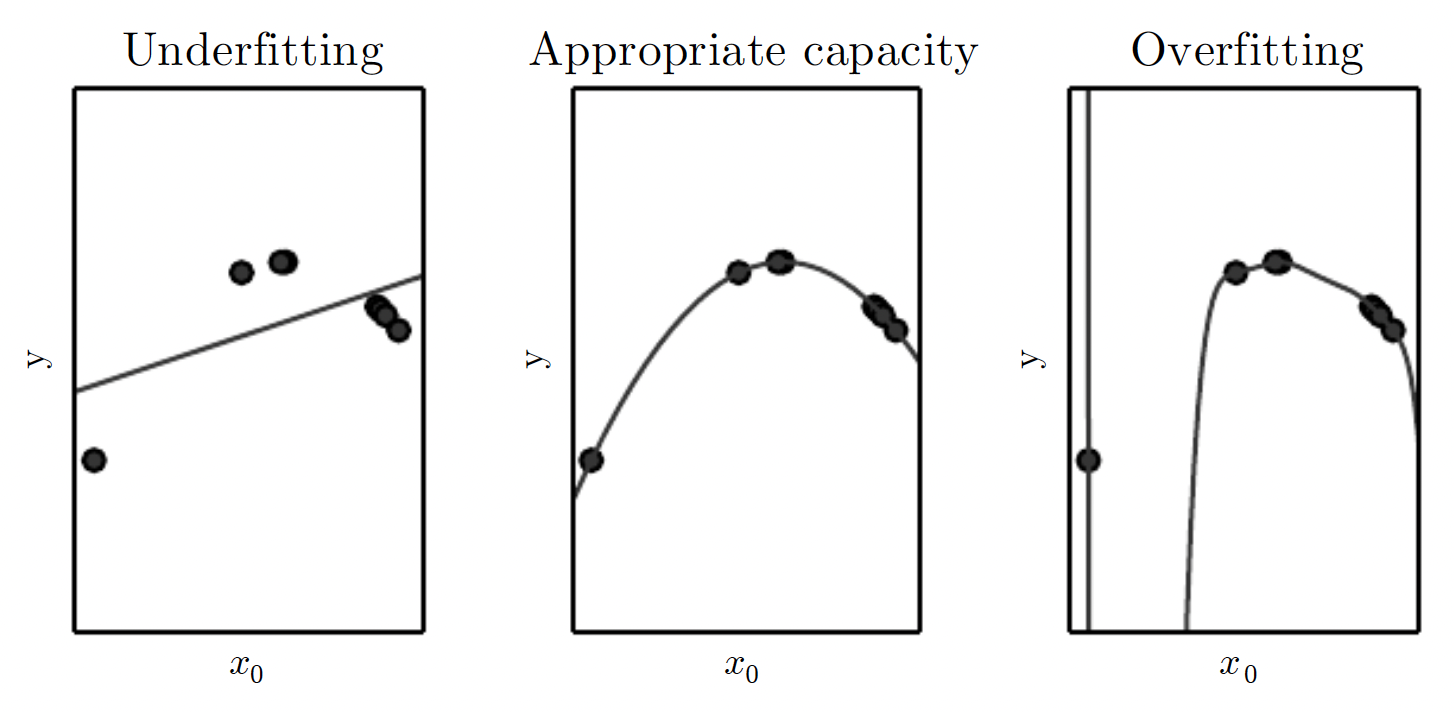
\includegraphics{fitting}
  \caption{Diagrams representing Underfitting, Appropriate, and Overfitting, from \citep{Goodfellow-et-al-2016}}
\end{figure}
  \subsection{Overfitting}%
  \label{sub:Overfitting}
\textbf{Overfitting} refers to the process of producing an analysis that matches a given set of data too closely, which can lead to problems when trying to fit new data or make reliable predictions about future events. That is, a mathematical model starts overfitting when it begins to memorize the data, rather than learn from it. 

In the topic of machine learning, if we choose too large of a network, it will behave like a lookup table on the data it was trained with, but won't generalize well to new data. Put another way, when a neural network has an excessive number of parameters, it can overfit, just like any other statistical model \citep{book:AIModernApp}.

As was hinted above, the degree of overfitting is influenced by the amount of data supplied, as well as the model's \textit{complexity}. The complexity of the model is determined by the number of underlying parameters that a neural network has. Additional degrees of freedom are the consequence of having more parameters, which can be utilized to explain certain training data points without making a strong generalization to new ones \citep{inbook:Aggarwal-4.1}.
\begin{wrapfigure}{R}{0.4\textwidth} %this figure will be at the right
    \centering
    \label{Overfitting}
    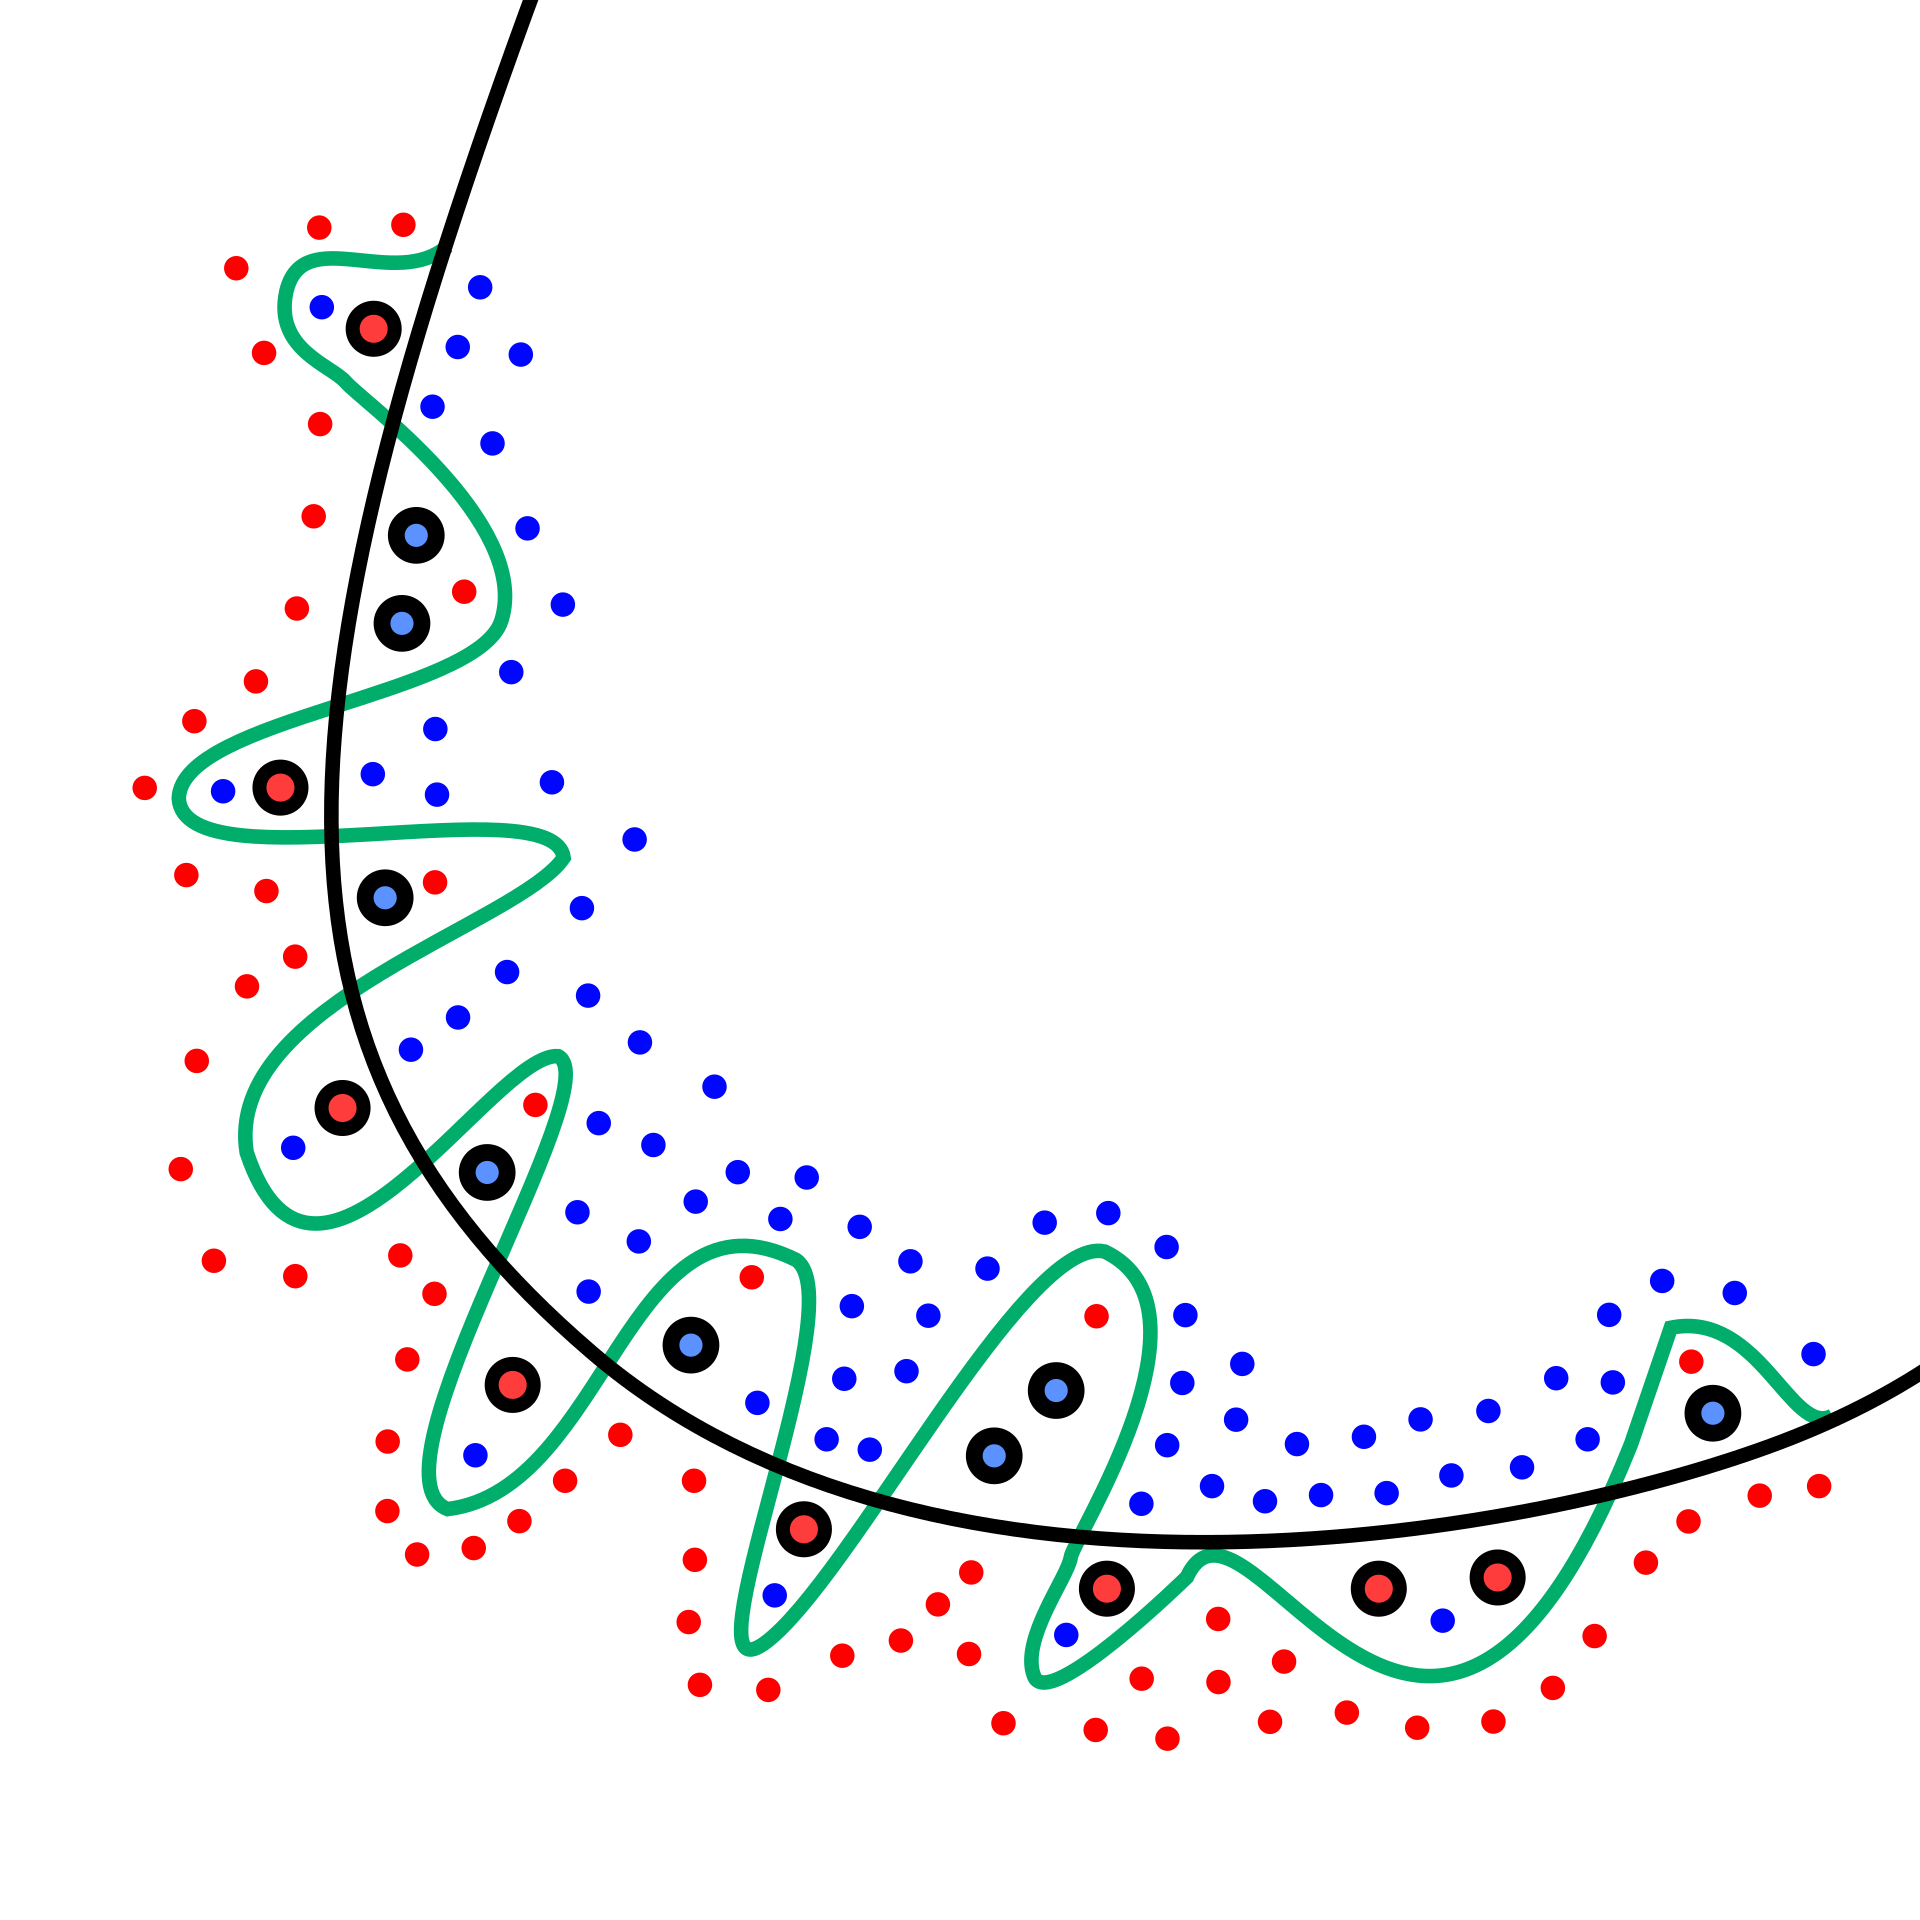
\includegraphics[width=0.4\textwidth]{Overfitting}
    \caption{A diagram showing overfitting (green line) of data from \citep{overfitting-img}}
\end{wrapfigure}
\begin{example}
  Suppose we have 5 training pairs $(x, t)$ available. Then, it can be shown that there exists a degree 4 polynomial that fits the 5 training points exactly with zero error. This does not mean, however, that the polynomial will approximate unseen data with zero error. 
\end{example}
As seen in figure \ref{Overfitting}, an overfit model will have low \textit{bias}, but high \textit{variance} on the training data. However, an overfit model will "have estimated (and actual) sampling variances that are needlessly large (the precision of the estimators is poor, relative to what could have been accomplished with a more parsimonious model) [...]. A best approximating model is achieved by properly balancing the errors of underfitting and overfitting." \citep{burnham2002model}.
\begin{remark} 
  In machine learning models, overfitting is more likely when learning is performed for too long, or when the training data set is small.
\end{remark}
\subsection{Underfitting}%
  \label{sub:Underfitting}
  Underfitting is essentially the inverse of overfitting. It occurs when a model is too basic, and lacks the complexity, i.e. the number of parameters, to explain the patterns in the data. An underfit model will have high bias and low variance on the training data, the exact opposite of an overfit model. In other words, underfitting is failing to learn enough from the training set. For instance, when fitting a linear model to non-linear data, under-fitting would happen. Such a model's predicting ability would be mediocre both for the training and testing data.

  Underfitting is not as widely discussed as overfitting, since it can be detected easily by evaluating how well the model is performing on the training data. 

 \subsection{Mastering the Fit}%
  \label{sub:Mastering the Fit}
  Now that we've shown how bad a Machine Learning algorithm can be, we'll show how to fix it. By changing a model's capacity, we may alter how likely it is to overfit, or underfit. 
  \begin{definition}[Capacity]
   We define the capacity of a model as its ability to fit a wide variety of
functions. Models with low capacity may struggle to fit the training set, while models
with high capacity can overfit by memorizing properties of the training set that do
not serve them well on the test set. The capacity of a model is a way to measure its complexity.
  \end{definition}

  Before altering the capacity of a model, one must evaluate whether a model is overfitting or underfitting. This can be done with the help of cross-validation, which we'll discuss in the next chapter.

  As long as the training error is low, one way to increase regularization without playing with capacity is to increase the amount of training data. If this is not possible, there are a number of components we can adjust in order to control the capacity of a model, such as \citep{capacity-Brownlee}, 
\begin{wrapfigure}{R}{0.4\textwidth} %this figure will be at the right
    \centering
    \label{capacity}
    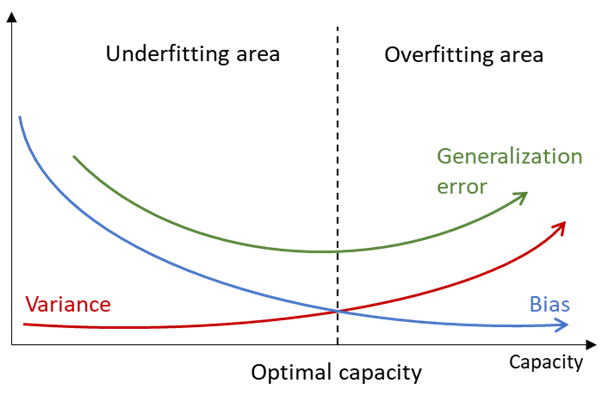
\includegraphics[width=0.4\textwidth]{capacity}
    \caption{A diagram showing the optimal capacity of a model and its relation with the \textit{bias-variance trade-off}, from \citep{capacity-Kowalik}}
\end{wrapfigure}
  \begin{enumerate}
    \item The number of nodes per layer (\textbf{width}) 
    \item The number of layers (\textbf{depth})
  \end{enumerate}
  It makes sense that augmenting these would increase the capacity, as they clearly increase the complexity of the model, which we know is closely related its capacity. It should be noted, however, that increasing the number of nodes and layers in a model can also increase its running time and memory usage. 

  Other ways to increase capacity include tuning the learning rate optimally, decreasing the \textit{weight decay coefficient}, and decreasing the \textit{dropout rate.} We refer the reader to chapter 11 of \cite{Goodfellow-et-al-2016} for more information on this topic.

  \subsection{Cross-Validation}%
  \label{sub:Cross-Validation}
Cross-validation is a technique that aims to test the ML model's testing capabilities on unseen data. This helps identify issues such as \textit{overfitting}, discussed above, or \textit{selection bias}, which is the result of selecting training data in a non-random way which doesn't represent the population. Cross-validation provides insight into how well the model will generalize to a different dataset.

The most common technique used is \textbf{k-fold cross-validation.} It allows one to repeatedly train and test the model $k$ times on various randomly chosen subsets of the training data. The average test error across $k$ trials can then be used to estimate the test error. In trial $i$, the $i^{th}$ subset of the data is used as the test set, and the remaining data is utilized as the training set. One issue is that there are no unbiased estimators of the variance of such average error estimators, but estimations are normally used \citep{Goodfellow-et-al-2016}. The following is the pseudo-code for the k-fold cross validation algorithm.


\begin{algorithm}[h!]
  \SetKwProg{Fn}{Function }{\string:}{}
  \SetKwFunction{KFoldXV}{KFoldXV}
  \caption{$k$-fold cross-validation}\label{k-CrossVal} 
  \Fn{\KFoldXV{$\mathbb{D}, A, L, k$}}{
  \textbf {Require: } $\mathbb{D}$ \text {, the given dataset, with elements } $ \boldsymbol{z}^{(i)}$\\
  \textbf {Require: } $A$, the learning algorithm, seen as a function that takes a dataset as input and outputs a learned function \\
  \textbf {Require:} $L$, the loss function, seen as a function from a learned function $f$ and an example $\boldsymbol{z}^{(i)} \in \mathbb{D}$ to a scalar $\in \mathbb{R}$\\
  \textbf {Require: } $k$ \text {, the number of folds }\\
  \BlankLine
  Split $\mathbb{D}$ into $k$ mutually exclusive subsets $\mathbb{D}_i$, whose union is $\mathbb{D}$\\
  \For{$i$ from 1 to $k$ }{
    $f_i = A(\mathbb{D}\ \mathbb{D}_i)$;\\
    \For{$z^{(j)}$ in $\mathbb{D}_i$ }{
      $e_j = L(f_i,z^{(j)} )$;
    }
  }
  \Return $e$;
  }
\end{algorithm}

\subsection{Regularization Techniques}%
  \label{sub:Regularization Techniques}

 \subsubsection{Early Stopping}%
  \label{sub:Early Stopping}

\subsubsection{L1 and L2 Regularization}    \label{sub:L1 and L2 Regularization}

\subsubsection{Dropout}%
  \label{sub:Dropout}
    \section{Conclusion}%
    \label{sec:Conclusion}
  As we've journeyed through the amazing realm of supervised machine learning, we've seen how powerful it can be, from the basic concept of neural networks, all the way to the more advanced method of backpropagation. It becomes evident, however, that the reliance of supervised learning on meticulously labeled datasets poses a significant limitation. The need for abundant, high-quality data, paired with corresponding inputs and desired outputs, can be restrictive and often impractical in real-world scenarios. This limitation becomes particularly apparent when faced with complex tasks where defining the desired outputs may be challenging or even impossible.

\newpage

 

 

{\footnotesize
  \bibliography{ML_Report_DRP2024}
}
%\bibliographystyle{apa} 
\bibliographystyle{plainnat}


%\bibliography{DeepRL}
%\bibliographystyle{iclr2017_conference}
%\bibliographystyle{apa}

\end{document} 

%ArXiv e-prints
